\documentclass[twocolumn]{article}
\usepackage[utf8]{inputenc}
\usepackage[skip=6pt, indent=0pt]{parskip}
\usepackage{graphicx}
\usepackage{tikz}
\usetikzlibrary{automata, positioning, arrows}

\title{CS 460 {-} Compilers}
\author{Arian Izadi}
\date{Spring 2024}

\begin{document}

\maketitle

\section{Languages}

Syntax is the rules for what a syntactically correct program looks like.
Semantics is the meaning of a program.

When does it matter the order of evaluation (right to left vs left to right)?
When the code has side effects, an example of this is postfix vs prefix increment (a++ vs ++a).

Compilers for a language L, move from front end $\to$ intermediate representation $\to$ back end.

\begin{itemize}
  \item Front end: Lexical Analysis, Syntax Analysis, and Semantic Analysis
  \item Intermediate: Intermediate Code
  \item Back end: Optimizer and Code Generation
\end{itemize}

\subsection{Lexical Analysis \& Scanning}

Lexical analysis, a scanner, is the process of converting a stream of characters into a stream of tokens.

\begin{enumerate}
  \item Find all terminals in the grammar.
  \item Write the Scanner.
        \begin{enumerate}
          \item Do we use a DFA, NFA, or PDA{?}
          \item Look at token types. All tokens can be expressed by a regular expression.
                \begin{enumerate}
                  \item Symbols: Semicolon, commas, etc.
                  \item Keywords: for, while, etc.
                  \item Variables: x, y, etc.
                  \item Numbers: 1, 3.14, 0{x}64, etc.
                \end{enumerate}
        \end{enumerate}
\end{enumerate}

\pagebreak

\paragraph*{Chomsky Language Hierarchy}

\begin{itemize}
  \item Type 0: Unrestricted (Turing Machines)
  \item Type 1: Context Sensitive
  \item Type 2: Context Free (PDA)
  \item Type 3: Regular Expressions (NFA, DFA)
\end{itemize}

Both RE and CFG have 1 non-terminal on the left of any combination of terminals and non-terminals on the right.

\textbf{Example 1:}

$S \to X \quad$
$X \to aXb | d \quad$
\hfill
not regular: $a^n d b^n$

\textbf{Example 2:}

$S \to X \quad$
$X \to aX | b \quad$
\hfill
regular: $a^* b$

\textbf{Example 3:}

$S \to X \quad$
$X \to aY | \epsilon \quad$
$Y \to bX \quad$
\hfill
regular: $(ab){^*}$

An NFA for recognizing tokens, construct NFA for each construct of RE\@.

$\mathcal{E}$:

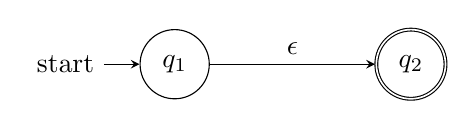
\begin{tikzpicture}[>=stealth, node distance=3cm, on grid, auto]
  \node[state, initial] (q1) {$q_1$};
  \node[state, accepting, right=of q1] (q2) {$q_2$};
  \path[->] (q1) edge node {$\epsilon$} (q2);
\end{tikzpicture}

$a \epsilon \Sigma$:

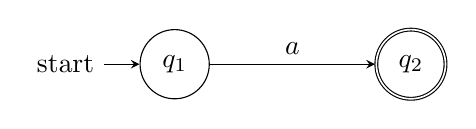
\begin{tikzpicture}[>=stealth, node distance=3cm, on grid, auto]
  \node[state, initial] (q1) {$q_1$};
  \node[state, accepting, right=of q1] (q2) {$q_2$};
  \path[->] (q1) edge node {$a$} (q2);
\end{tikzpicture}

\pagebreak

% $s | t$:

% \begin{tikzpicture}[>=stealth, node distance=2cm, on grid, auto]
%   \node[state, initial] (q1) {$q_1$};
%   \node[state, right=of q1] (q2) {$q_2$};
%   \node[state, accepting, right=of q2] (q3) {$q_3$};
%   \node[state, below=of q2] (q4) {$q_4$};

%   \path[->] (q1) edge node[above] {$\epsilon$} (q2);
%   \path[->] (q2) edge node[above] {$\epsilon$} (q3);
%   \path[->] (q1) edge node[left] {$\epsilon$} (q4);
%   \path[->] (q4) edge node[right] {$\epsilon$} (q3);
% \end{tikzpicture}


Any RE can be turned into an NFA using these rules.
If all the tokens of a language are represented by RE's, $r_1, \dots, r_n$.
Create an NFA for each RE\@.


\end{document}